% chktex-file 44 32 36 38 18 11 8 26

\pagestyle{DS_FP}
%\NomPrenomNote{}

\bigskip

\section*{PARTIE A~--~Fiabilité d'un parc de passerelles LoRaWAN (Probabilités)}

\medskip

\emph{Dans cette partie, vous arrondirez toutes les valeurs à $10^{-4}$ si nécessaire.}

\medskip

 \begin{minipage}{0.48\textwidth}
le stock est composé de:
\begin{itemize}
    \item $75\%$ de passerelles de type \textbf{Alpha} dont $2\%$ présentent un défaut de synchronisation.
    \item $25\%$ de passerelles de type \textbf{Beta} dont $6\%$ présentent un défaut de synchronisation.
\end{itemize}

On note 
\begin{itemize}
    \item $D$ l'événement « la passerelle est défectueuse ».
    \item $A$ l'événement « la passerelle est de type Alpha ».
    \item $B$ l'événement « la passerelle est de type Beta ».
\end{itemize}


Une passerelle est prélevée au hasard en sortie de chaîne.

\medskip

\begin{enumerate}[series=monDS, resume]
    \item Compléter l'arbre de probabilité ci-contre.
\end{enumerate}

\end{minipage}\hfill{}
\begin{minipage}{0.48\textwidth}
    \begin{blocvisiblex}[height=6]
    {\begin{center}
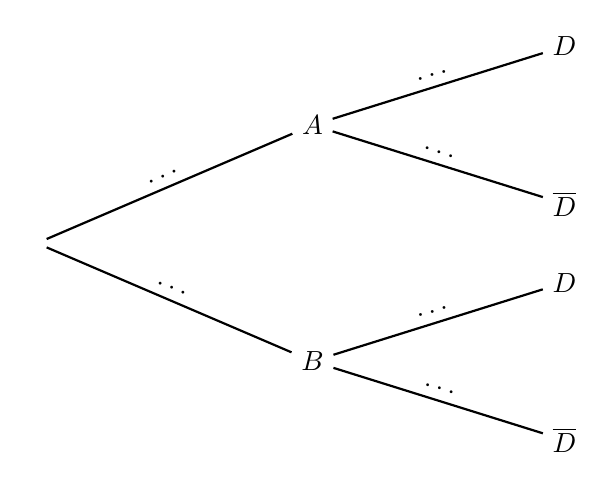
\begin{tikzpicture}[
    grow=right,     % On définit la croissance vers la droite
    % Réglages des distances entre les niveaux et les branches
    level 1/.style={sibling distance=3cm, level distance=3.5cm},
    level 2/.style={sibling distance=2cm, level distance=3.2cm},
    every node/.style={sloped}, % Aligne le texte sur les branches
    edge from parent/.style={draw, thick} % Ajoute une flèche au bout
]
% Racine
\node {} 
    child { node {$B$}
        child { node {$\overline{D}$} 
            edge from parent node[above] {$\ldots{}$} }
        child { node {$D$} 
            edge from parent node[above] {$\ldots{}$} }
        edge from parent node[above] {$\ldots{}$} }
    child { node {$A$}
        child { node {$\overline{D}$} 
            edge from parent node[above] {$\ldots{}$} }
        child { node {$D$} 
            edge from parent node[above] {$\ldots{}$} }
        edge from parent node[above] {$\ldots{}$} }
    ;
\end{tikzpicture}
\end{center}}
\begin{center}
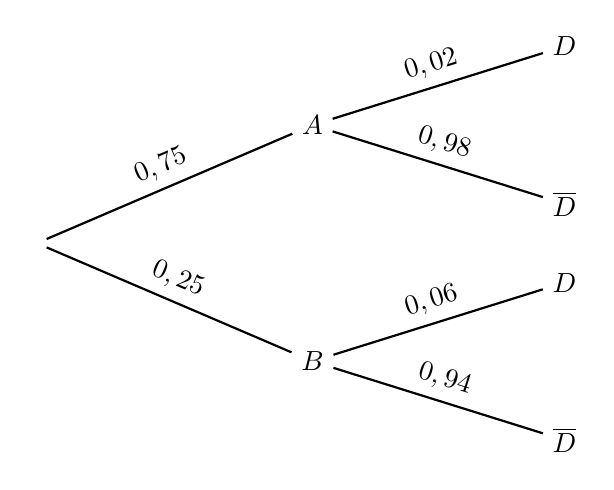
\begin{tikzpicture}[
    grow=right,     % On définit la croissance vers la droite
    % Réglages des distances entre les niveaux et les branches
    level 1/.style={sibling distance=3cm, level distance=3.5cm},
    level 2/.style={sibling distance=2cm, level distance=3.2cm},
    every node/.style={sloped}, % Aligne le texte sur les branches
    edge from parent/.style={draw, thick} % Ajoute une flèche au bout
    %edge from parent/.style={draw, -latex, thick} % Ajoute une flèche au bout
]
% Racine
\node {} 
    child { node {$B$}
        child { node {$\overline{D}$} 
            edge from parent node[above] {$0,94$} }
        child { node {$D$} 
            edge from parent node[above] {$0,06$} }
        edge from parent node[above] {$0,25$} }
    child { node {$A$}
        child { node {$\overline{D}$} 
            edge from parent node[above] {$0,98$} }
        child { node {$D$} 
            edge from parent node[above] {$0,02$} }
        edge from parent node[above] {$0,75$} }
    ;
\end{tikzpicture}
\end{center}
    \end{blocvisiblex}
\end{minipage}



    
\begin{enumerate}[resume=monDS]
    \item Calculer la probabilité que la passerelle prélevée soit défectueuse et soit de type \textbf{Alpha}.
     \begin{blocvisiblex}[height=1.5]
    {\quad}
    $P(A\cap D)=P(A) \times P_D(A)=0,75 \times 0,02=0,015$

    \smallskip
    La probabilité que la passerelle soit défectueuse et soit de type \textbf{Alpha} est de $0,015$.
     \end{blocvisiblex}
     \medskip
    \item Calculer la probabilité que la passerelle prélevée soit défectueuse.
    \begin{blocvisiblex}[height=1.5]
    {\quad}
    $P(D)=P(A\cap D)+P(B\cap D)=P(A) \times P_D(A)+P(B) \times P_D(B)=0,75 \times 0,02+0,25 \times 0,06=0,03$

        \smallskip
    La probabilité que la passerelle soit défectueuse est de $0,03$.
    \end{blocvisiblex}
    \medskip
    \item Sachant que la passerelle est défectueuse, calculer la probabilité qu'elle soit de type \textbf{Alpha}.
    \begin{blocvisiblex}[height=2]
    {\quad}
    $P_A(D)=\dfrac{P(A\cap D)}{P(D)}=\dfrac{P(A) \times P_D(A)}{P(D)}=\dfrac{0,75 \times 0,02}{0,03}\approx 0,5$

        \smallskip
    La probabilité que la passerelle soit de type \textbf{Alpha} sachant qu'elle est défectueuse est $0,5$.
     \end{blocvisiblex}
     \medskip
    \item  On prélève un lot de 30 passerelles de manière indépendante. Soit $Y$ la variable aléatoire comptant le nombre de passerelles défectueuses. Démontrer que $Y$ suit une loi binomiale dont on précisera les paramètres.
    \begin{blocvisiblex}[height=3.5]
    {\quad}
    \begin{itemize}
        \item "choisir une passerelle défectueuse" est une expérience à deux issues: "la passerelle est défectueuse" de $p=0,03$ et "la passerelle n'est pas défectueuse" de $p=0,97$
        \item On répète cette expérience $n=30$ fois de manière identique et indépendante
        \item $Y$ compte le nombre de succès (passerelles défectueuses) parmi les 30 expériences
        \item Donc $Y$ suit une loi binomiale de paramètres $n=30$ et $p=0,03$.
    \end{itemize}
    \end{blocvisiblex}
        \medskip
        \item Calculer la probabilité d'avoir au moins 2 passerelles défectueuses dans ce lot.
    \begin{blocvisiblex}[height=1.5]
    {\quad}
    $P(Y\geq 2)\approx 0,2269$

        \smallskip
    La probabilité d'avoir au moins 2 passerelles défectueuses dans ce lot est d'environ $0,2269$.
    \end{blocvisiblex}
    \medskip

    \pagebreak

    \item Calculer la probabilité d'avoir exactement 3 passerelles défectueuses dans ce lot.
    \begin{blocvisiblex}[height=1.5]
    {\quad}
    $P(Y=3)\approx 0,0447$

        \smallskip  
    La probabilité d'avoir exactement 3 passerelles défectueuses dans ce lot est d'environ $0,0482$.
    \end{blocvisiblex}
    \medskip
    \item Combien faut-il prélever de passerelles pour que la probabilité d'avoir au moins 1 passerelle défectueuse soit supérieure à 20\% ? Déterminer à l'aide de Géogébra à partir de quelle valeur de $n$ la condition est satisfaite.
    \begin{blocvisiblex}[height=2]
    {\quad}
    $P(Y\geq 1)=1-P(Y=0)=1-\binom{n}{0} \times 0,03^0 \times (1-0,03)^n = 1-(1-0,03)^n=1-0,97^n$  

    Il faut prélever au moins 8 passerelles pour que la probabilité d'en avoir au moins 1 défectueuse soit supérieure à 20\%.
    \end{blocvisiblex}
     \end{enumerate}


\section*{PARTIE B~--~Étude de l'attenuation d'un signal audio (Fonctions)}

Pour protéger les composants d'un amplificateur, on étudie le gain $f$ d'un circuit de filtrage en fonction de la fréquence $x$ (en kHz).
On considère la fonction $f$ définie sur $\ff{1}{20}$ par:

\fbox{$f(x)=a x-b \ln(x)$} \quad $f(x)$ représente le gain en dB pour une fréquence $x$. $a$ et $b$ sont des constantes réelles.

\begin{itemize}
    \item Le gain est minimal pour une fréquence de 2 kHz
    \item Le gain pour une fréquence de 1 kHz est de 5 dB.
\end{itemize}

 \begin{enumerate}[resume=monDS]

        
    \item Déterminer à l'aide de Géogébra les valeurs de $a$ et $b$. \hfill\reponseLigne[5cm]{\texttt{$a=5$ et $b=10$}} 

\end{enumerate}

 On décide de modéliser le gain par la fonction $f$ définie sur $\ff{1}{20}$ par \fbox{$f(x)=5(x-2\ln(x))$}

 \begin{enumerate}[resume=monDS]

        \item Calculer $f'(x)$ 
        \begin{blocvisiblex}[height=1.5]
        {\quad} 
        $f'(x)=5\left(1-\dfrac{2}{x}\right)= 5 - \dfrac{10}{x}=\dfrac{5x-10}{x}$
        \end{blocvisiblex}

        \medskip
        \item En déduire les variations de $f$ sur $\ff{1}{20}$.
        \begin{blocvisiblex}[height=2.5]
        {\quad}
        $f'(x)$ est strictement négative sur $\ff{1}{2}$, ainsi $f$ est strictement décroissante sur $\ff{1}{2}$.

        $f'(x)$ est strictement positive sur $\ff{2}{20}$, ainsi $f$ est strictement croissante sur $\ff{2}{20}$.
         \end{blocvisiblex}

         \medskip
         \item On considère que le signal est "coupé" lorsque le gain devient inférieur à $3,5$ dB. Déterminer à l'aide de Géogébra pour quelles fréquences le signal est coupé.
            \begin{blocvisiblex}[height=1.2]
            {\quad}
            Le signal est coupé sur $\ff{1,47}{2,65}$
             \end{blocvisiblex}

             \medskip


             \item Déterminer une primitive $F$ de la foncton $f$.
                \begin{blocvisiblex}[height=1.5]
                {\quad}
                $F(x)=\dfrac{5}{2}x^2-10(x\ln(x)-x)$
                 \end{blocvisiblex}

                 \medskip
                 \item Calculer le gain moyen du circuit sur la plage de fréquence $[1;3]$ arrondi à $10^{-2}$ près.
                    \begin{blocvisiblex}[height=1.5]
                    {\quad}
                    Le gain moyen du circuit sur la plage de fréquence $[1;3]$ est de $\dfrac{1}{3-1}\int_1^3 f(x) \, \dx\approx 3,52$ dB.
                     \end{blocvisiblex}
            
    \end{enumerate}


\medskip

    \section*{PARTIE C~--~Décharge d'une batterie de secours (Suites)}

Lors d'une coupure de courant, une batterie de secours alimente un serveur. Sa capacité initiale est de 800 Wh. Chaque heure, elle perd $12\%$ de l'énergie qu'il lui reste.

Soit $u_n$ l'énergie restante (en Wh) après $n$ heures.

\begin{enumerate}[series=monDS, resume]
    \item Justifier que la suite $(u_n)$ vérifie la relation de récurrence $u_{n+1}=0,88\cdot u_n$.
    \begin{blocvisiblex}[height=3.5]
    {\quad}
    La suite $(u_n)$ vérifie la relation de récurrence $u_{n+1}=0,88\cdot u_n$ car à chaque heure, la batterie perd $12\%$ de l'énergie qu'elle lui reste.

    On a donc $u_{n+1}=u_n-0,12\cdot u_n=0,88\cdot u_n$.

    \end{blocvisiblex}
    \medskip
    \item Déterminer la nature de la suite $(u_n)$. 
    \begin{blocvisiblex}[height=2]
    {\quad}

    La suite $(u_n)$ est de la forme $u_{n+1}=q \times u_n$ avec $q=0,88$ constant, donc c'est une suite géométrique de raison $0,88$ et de premier terme $u_0=800$.
    \end{blocvisiblex}
    \medskip
    \item Exprimer $u_n$ en fonction de $n$. 
    \begin{blocvisiblex}[height=1.5]
    {\quad}
    $(u_n)$ est une SG de raison $0,88$ et de premier terme $u_0=800$, donc pour tout $n$ entier naturel, on a $u_n=u_0 \times q^n=800 \times 0,88^n$.
    \end{blocvisiblex}
    \medskip
    \item Compléter le script suivant pour déterminer après combien d'heures l'énergie sera inférieure à 100 Wh.
    

    \begin{tcblisting}{%
  listing only,
  colback=white, 
  colupper=black, 
  title=Algorithme de recherche de seuil,
  boxsep=0pt,
  left=5mm,
  listing options={
    numbers=none,
    basicstyle=\ttfamily,
    escapeinside={(*}{*)},
    literate={<-}{{$\bm{\leftarrow}$}}2, % Ajout d'un petit espace après la flèche
    frame=none % Supprime le cadre interne de listings
    }
}
n <- 0
u <- 800
tant que (*\trou{u >= 100}*):
        u <- (*\trou{0,88 * u}*)
        n <- (*\trou{n + 1}*)
afficher (n)
\end{tcblisting}

\item Déterminer par la méthode de votre choix après combien d'heures l'énergie sera inférieure à 100 Wh.
\begin{blocvisiblex}[height=1.5]
{\quad}
On cherche à déterminer le plus petit entier naturel $n$ tel que $u_n<100$. 
On trouve $n=17$ donc après 17 heures, l'énergie sera inférieure à 100 Wh.
\end{blocvisiblex}

\end{enumerate}

\pagebreak

\thispagestyle{DS_LP}
\section*{PARTIE D: Pour aller plus loin}


\subsubsection*{Comparaison de deux modèles de décharge}

Une autre batterie (Modèle Gamma) suit une décharge linéaire. Sa capacité initiale est de 800 Wh et elle perd 60 Wh chaque heure. 

\begin{enumerate}[series=monDS, resume]
    \item Déterminer l'énergie restante après $n$ heures pour ce modèle de batterie.
    \begin{blocvisiblex}[height=1]
    {\quad}
    $(w_n)$ est une suite définie par $w_n=800-60n$ pour tout entier naturel $n$.
    \end{blocvisiblex}
    \medskip
    \item Déterminer après combien d'heures l'énergie de ce modèle de batterie sera inférieure à 100 Wh.
    \begin{blocvisiblex}[height=1.5]
    {\quad} 
    On cherche à déterminer le plus petit entier naturel $n$ tel que $w_n<100$.
    On a $w_n=800-60n<100 \Leftrightarrow 60n>700 \Leftrightarrow n>11,67$.
    Ainsi, après 12 heures, l'énergie de cette batterie sera inférieure à 100 Wh.
    \end{blocvisiblex}
    \medskip
    \item Déterminer à l'aide de Géogébra à partir de quelle heure le modèle Gamma devient moins avantageux que le modèle de la partie C.
    \begin{blocvisiblex}[height=1.]
    {\quad}
    Le modèle Gamma devient moins avantageux que le modèle de la partie C à partir de la 10ème heure.
    \end{blocvisiblex}
    \end{enumerate}


    \subsubsection*{Analyse de performance}

    On étudie le temps de latence $L(n)$ d'un réseau en fonction du nombre $n$ de paquets envoyés, modélisé par : $L(n)=20\times(1-\e^{-0,1n})$
    
    \begin{enumerate}[resume=monDS]
        \item Déterminer la limite de $L(n)$ quand $n$ tend vers $+\infty$.
            \begin{blocvisiblex}[height=1.5]
    {\quad}
    La limite de $L(n)$ quand $n$ tend vers $+\infty$ est égale à $20$ ms.
    \end{blocvisiblex}
        \medskip
    \end{enumerate}
         On considère que le réseau est saturé quand la latence dépasse $95\%$ de sa valeur limite.

            \begin{enumerate}[resume=monDS]

    \item Déterminer à partir de quel nombre de paquets $n$ le réseau est considéré comme saturé.
    \begin{blocvisiblex}[height=1.]
    {\quad}
    $L(n)>19 \Leftrightarrow n>29,96$.
    Ainsi, le réseau est considéré comme saturé à partir de 30 paquets envoyés.
    \end{blocvisiblex}
    \end{enumerate}

    
\subsubsection*{Etude du régime transitoire}

La tension $u(t)$ au bornes de la batterie de secours à l'instant $t$ (en heures) est modélisée par la fonction $u$ définie sur $\ff{0}{+\infty}$ qui est solution de l'équation: \fbox{$u'(t)+0,5u(t)=10$}

On suppose que $u(t)$ est de la forme $u(t)=e^{kt}+C$ où $k$ et $C$ sont des constantes réelles.

\begin{enumerate}[resume=monDS]
    \item Tracer la courbe représentative de $u$ sur géogébra.
    \item Tracer la courbe représentative de la fonction $g$ définie sur $\ff{0}{+\infty}$ par $g(t)=u'(t)+0,5u(t)$ sur géogébra.
    \item Déterminer les valeurs de $k$ et $C$ afin que $g(t)=10$ pour tout $t$ de $\ff{0}{+\infty}$.
    \begin{blocvisiblex}[height=2.5]
    {\quad}
    $u(t)=e^{kt}+C$ est solution de l'équation différentielle $u'(t)+0,5u(t)=10$ si $k=-0,5$ et $C=20$ car $u'(t)=ke^{kt}$ et $u'(t)+0,5u(t)=ke^{kt}+0,5(e^{kt}+C)=(k+0,5)e^{kt}+0,5C=10$ si $k=-0,5$ et $C=20$.
    \end{blocvisiblex}


\end{enumerate}





\end{document}
    \end{minipage}
    \medskip

    \end{enumerate}

\bigskip



